\section{Initialization}
The number of particles $N$ is given by $4M^3$, where $M$ is the number of unit cells per dimension. Using the density $\rho$ and $N$, the dimensions of the box are determined and filled with unit cells. Four particles are then placed in each unit cell corresponding to an fcc Bravais lattice structure with lattice constant $a=L/M$. Overlapping particles are avoided by filling each unit cell with only the lower left four particles, as shown in figure \ref{fig:unit_cell}. All particles are then displaced by a distance $a/10$ in each direction to avoid ambiguities in the periodic boundary conditions. This distribution will be relatively close to a stable distribution for the Lennard-Jones potential, reducing the amount of timesteps needed before the system will equilibrate.
\begin{Figure}
 \centering
 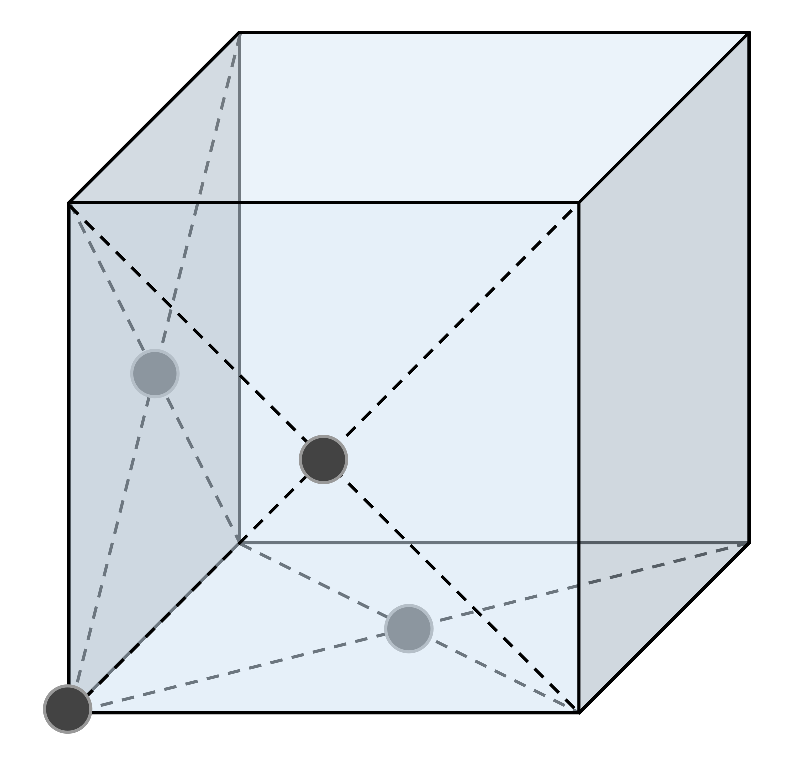
\includegraphics[width=0.35\linewidth]{fcc_cell.eps}
 \captionof{figure}{fcc Bravais unit cell.}\label{fig:unit_cell}
\end{Figure}

The particles are given an initial velocity with a Maxwell distribution\cite{jos}. The velocities are then renormalized by setting the centre of mass velocity to zero and rescaling the velocities to fit with the desired temperature. This is done by comparing the current kinetic energy and the expected kinetic energy for the desired temperature according to the equipartition theorem. This means that all the velocities are rescaled uniformly by a factor

\begin{gather*}
\lambda = \sqrt{\frac{3\left(N-1\right)k_bT_d}{\sum_{i=1}^Nmv_i^2}}.
\end{gather*}

%The initialization functions are combined in 